\documentclass{article}
%\documentclass[2pt,english]{article}

\usepackage{cite}
\usepackage{listings}
%\usepackage{times}
\usepackage{color}
\usepackage{url}
\urlstyle{same} % Used for formatting formatting url footnotes
\usepackage{soul} % highlighting
\usepackage{forloop} % Project timeline
\usepackage{tabularx} % table text width
\usepackage{xcolor,colortbl} %%% Color Table Header
\usepackage{fancyhdr} % Header
%\usepackage{framed}		% Allows drawing text boxes
\usepackage{pgfgantt}
\usepackage{enumitem} % Use for enumerating A, B, C etc...

%Use a font size no smaller than 11 point and one inch margins.


\usepackage{xspace} % Needed for et al.
\newcommand{\etal}{{et al.\@\xspace}}

% Addressing Decision-Making Uncertainty in Self-Adaptive Systems By Accounting for Tactic Volatility
\newcommand{\Title}{Applying Dynamic Bayesian Matrix Factorization to Predict Tactic Volatility in Self-Adaptive Systems}

% Bayesian to Predict Tactic Volatility

\title{\Title} 


%\title{Reducing Tactic Latency Uncertainty in Self-Adaptive Systems}


\author{
	TPOC: Daniel E. Krutz and Qi Yu; \{dxkvse, qi.yu\}@rit.edu\\
%	Assistant Professor\\ % Removed for space
%	Rochester Institute of Technology\\
%	Department of Software Engineering \& Center of Cybersecurity \\
%	Mailing Address: 134 Lomb Memorial Drive \\
%	Rochester, NY 14623-5608 \\
%	Voice: 585-475-2896 \\
}
 \date{} % Remove the date

% Alter these values based on the actual length.
% The paper should be ~3 pages
%\usepackage[top=.3in, bottom=1in, left=1in, right=1in]{geometry} %% Changes the margins of the pages - This was breaking the header functions

\usepackage[bottom=1in, left=1in, right=1in, top=.3in]{geometry} %% Use this to make the page wider

\newcommand{\todo}[1]{\textcolor{cyan}{\textbf{[#1]}}}
%\newcommand{\XXX}[1]{\textcolor{green}{{\it [XXXX says: #1]}}}
%\newcommand{\XXX}[1]{\textcolor{yellow}{{\it [XXXX says: #1]}}}
\newcommand{\dan}[1]{\textcolor{blue}{{\it [Dan says: #1]}}}
\newcommand{\qi}[1]{\textcolor{red}{{\it [Qi says: #1]}}}
\newcommand{\xx}[1]{\textcolor{orange}{{\it [xx: #1]}}}


\pagestyle{fancy}
\lhead{\Title} % Leave empty to keep sections from being shown
\rhead{Daniel E. Krutz}

\usepackage{lastpage}
%\cfoot{\thepage\ of \pageref{LastPage}}



\begin{document}

\maketitle
\vspace{-10mm}
\section{Introduction}
\vspace{-2mm}

% Put something in about including uncertainty reduction tactics

Self-adaptive systems autonomously react to changing situations through \emph{tactics} (decisions). Example tactics include a cloud activating an additional virtual machine when the workload reaches a defined threshold, or a self-driving car deciding whether or not it needs to stop when a possible obstacle is encountered. These tactics frequently contain volatility in the form of the time necessary to perform the action, availability of the action, or dependability of the action. This volatility can substantially impact the decision-making process. Unfortunately, current self-adaptation techniques cannot account for real-world volatility during the decision-making process. This can negatively impact the system's efficiency, resiliency, and ability to complete mission objectives. To address this challenge, \ul{we present a Tactic Volatility Aware (TVA) approach that accounts for volatility in the decision-making process of self-adaptive/autonomous systems through the use of a dynamic Bayesian matrix factorization model.} This will \textbf{increase the system's resiliency, efficiency, and ability to complete mission-critical operations.} TVA is innovative as existing techniques are unable to consider tactic volatility in the decision-making process. %We will achieve project this with the following tasks:

\vspace{-2mm}
\section{Motivating Example}
\vspace{-2mm}
%% DK: Should the example be more focused on large or small UAVs? - What are they more interested in?
In this scenario, an autonomous UAV has the objective of collecting information on suspected enemy combatants when they are identified. The camera has an anticipated preparation time of .2 seconds. However, due to a mechanical issue, it has been taking .4 seconds to prepare the camera. In existing self-adaptive techniques, the system will be unable to learn about this latency volatility from previous experiences, and will be therefore unable to account for this unanticipated additional latency time. Our Tactic Volatility Aware (TVA) process will enable the system to learn from prior experiences and account for this volatility.

%Figure~\ref{fig:UAVLatencyExampleCamera} represents a scenario where 

\begin{figure}[h]
	\centering
    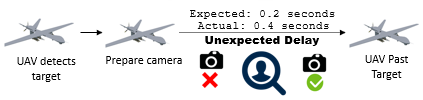
\includegraphics[scale=0.85]{images/UAVLatencyExampleCamera.png}
    \caption{Detrimental Impact of Unexpected Latency on Autonomous UAV}
    \label{fig:UAVLatencyExampleCamera}
\end{figure}

\vspace{-5mm}
\section{Proposed Tactic Volatility Aware (TVA) Solution}

We will develop a {\bf Bayesian dynamic matrix factorization model that jointly predicts multiple correlated tactic volatility parameters}, including latency, dependability, and availability. The joint prediction model assumes that there are a number of common factors, including both observable and latent, that affect these parameters. However, they may play a different role over different parameters. We will begin by modeling the latent factors and their contribution to the parameter of interest. 

%% Not sure if this should be included.
%Autonomous systems must frequently operate in new environments with little empirical data. To address this challenge, we will include the use of \emph{uncertainty reduction tactics} with the specific intent of data gathering

%\dan{Qi: Feel free to add to this? We can obviously chat about this in person.}


Our Tactic Volatility Aware solution will be easy to incorporate into popular self-adaptation loops such as MAPE-K, making it readily adoptable by a wide range of autonomous devices. Our Tactic Volatility Aware solution offers several advantages over existing decision-making systems that are unable to consider real-world tactic volatility:

\begin{enumerate}[noitemsep]
	\item Remedy inaccurate decision volatility determinations made by humans.
    \item Enable systems to make more accurate decisions, leading to more resilient autonomous devices that are better suited to complete desired mission objectives.
    \item Account for variations in volatility through calculated standard deviation in observed tactics.
	\item Improve system predictability.
%	\item Enable systems to complete mission and safety critical operations by accounting for tactic volatility.
%    \item Ability to update the expected decision volatility values through observing decision-making variability in the system.
%	\item Enable human engineer to define the maximum allowed decision-making latency to protect against decision latency that is outside of the defined maximum threshold.


\end{enumerate}



\end{document}


% Possible calls
% 	https://www.grants.gov/web/grants/view-opportunity.html?oppId=307829



